\chapter{Method}
\label{chap:method}

% intro: what data I needed
% materials
% the microscope and the detector
% analysis in AZtec
% extracting the data (data and k-factors?)
% analysis in HyperSpy
% my data treatment
% calibration
% background subtraction
% area under the peaks
% data from Mar(?)



The data needed in this project was SEM EDS spectra.
The spectra were acquired on a SEM APREO at NTNU NanoLab.
The spectra were from a sample containing different sections with different elements to get different spectra to work with.
The relevant material for data extraction is available on the GitHub repository for this project (ref).
The data is also available on the GitHub repository for this project, under the folder \verb|data/2022-09-06_EDS-Apreo|.
This method chapter describes the material used, the microscope and detector, and then the data processing.
The data processing starts with the analysis in AZtec and HyperSpy, and then presents the self made post data treatment.



%
%
\section{Materials and specimen}
\label{sec:method:materials}
% \ton{Can I use the results I have? E.g. GaAs? Do I need the TED Palla sample data before the master?}
EDS data was collected on one specimen with sections containing different materials.
A 300 \textmu m 2" Si wafer was cut in half and mounted with Cu tape on an FIB stub.
On the Si wafer a smaller piece of a GaAs wafer was mounted with Cu tape.
A Mo disk was mounted to the Si wafer with Ag paint.
In the middle of the Mo disk there was a hole where a TEM grid was mounted.
The TEM grid had GaAs nanowires on it, and the grid was made of Mo with C film.
Growth of the GaAs nanowires is described in \cite[Ch. 3]{skomedal_improving_2022}.
A schematic of the sample is shown in \cref{fig:method:materials:sample1}.

Six areas on the specimen was sampled, and their respective spectra are named: GaAs, Mo, (GaAs) NW, Si, Cu and Al.
GaAs is a piece of a GaAs wafer, where the Ga and As are 1:1.
Mo is a Mo disk.
(GaAs) NW is a Cu TEM 300 mesh grid with holey C film, where GaAs nanowires were grown by Au droplets, sometimes referred to as NW and sometimes as GaAs NW.
Si is the Si wafer.
Cu is the Cu-tape.
Al is the Al FIB stub.


% insert figure Materials-sample1.png
\begin{figure}[ht]
    \centering
    \colorbox{white}{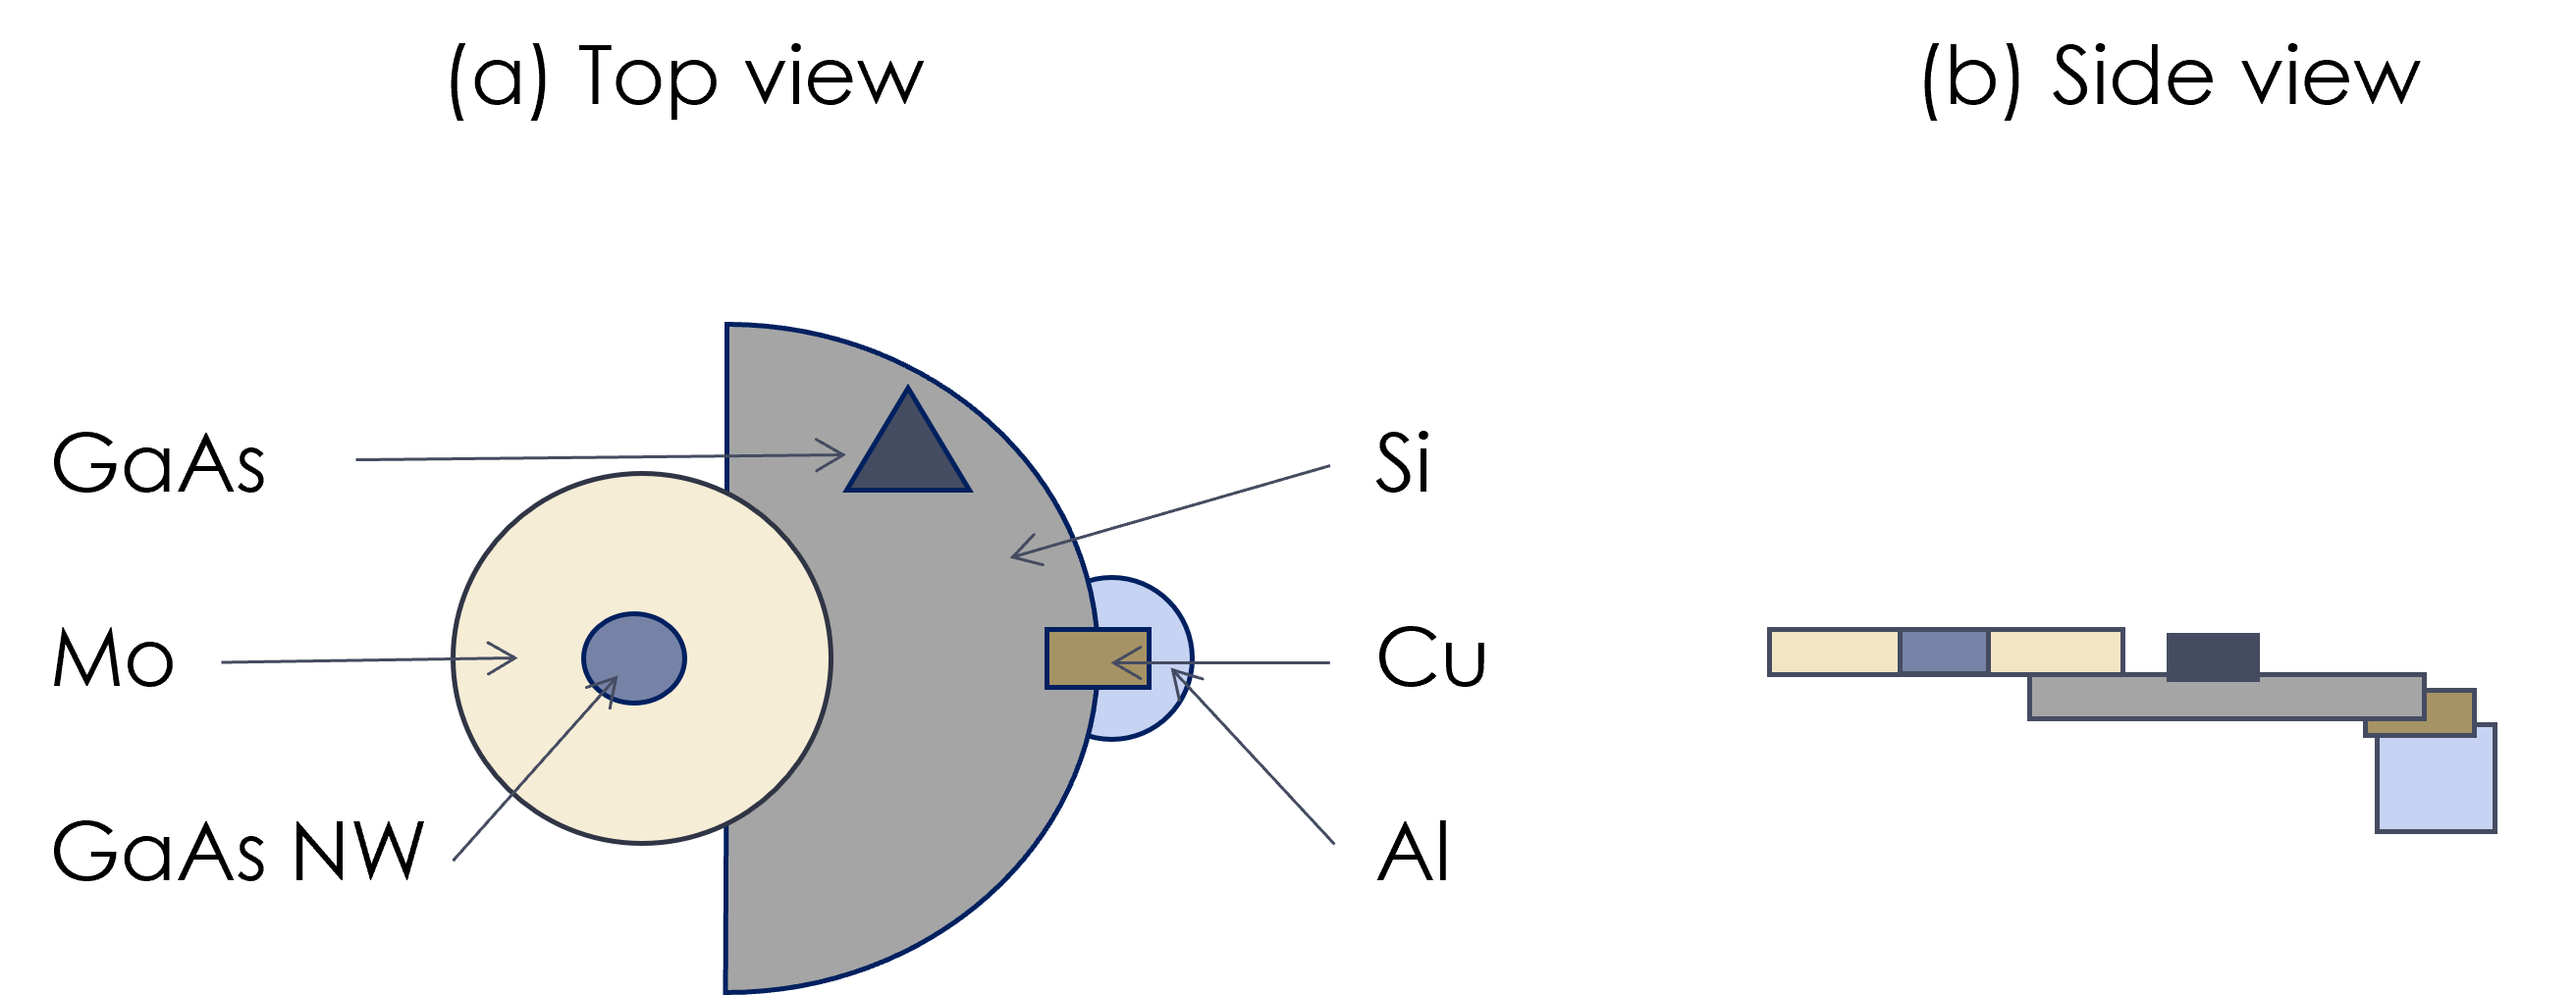
\includegraphics[width=0.8\textwidth]{figures/Materials-sample1.png}}
    \caption{
        The sample used for the EDS data collection in the SEM Apreo.
        (a) is top view and (b) is side view.
        GaAs is a piece of a GaAs wafer.
        Mo is a Mo disk.
        GaAs NW is the TEM grid of Mo with C film and GaAs nanowires.
        Si is the Si wafer.
        Cu is the Cu tape.
        Al is the Al FIB stub.
        % Ton: delete the below, can add to body text.
        % Four spectra with different $V_\textnormal{acc}$ was collected on the GaAs, Mo, Si, and GaAs NW.
        % Three spectra was taken on the Cu tape and one spectrum on the Al FIB stub.
    }
    \label{fig:method:materials:sample1}
\end{figure}



%
%
\section{The microscope and the detector}
\label{sec:method:detector}
The data was collected with the SEM Apreo from FEI with an Oxford EDX detector at NTNU NanoLab.
The detector is an EDX Oxford Xmax 80 mm$^2$ detector, with reported energy resolution of 127 eV \cite{oxford_xmax_80}.
The acceleration voltage, $V_\textnormal{acc}$, can be set from 0.2 to 30 kV.
In this project the $V_\textnormal{acc}$ was set to 5, 10, 15, and 30 kV.
The beam current, $I_\textnormal{beam}$, has a maximum value of 400 nA.
In this project the $I_\textnormal{beam}$ was set to 0.2, 0.4, 0.8, and 1.6 nA.
The SEM has an adjustable working distance.
The SEM is equipped with a BSE and a SE detector.

% my settings
The data collection was done on 5, 10, 15, and 30 kV.
The beam current was 0.2, 0.4, 0.8, or 1.6 nA, depending on the dead time of the detector, trying to get the dead time around 30\%.
% Below is moved to discussion
% Dead time at around 30\% was recommended by the supervisor of this project, Antonius T. J. von Helvoort, and is well below the problematic dead time of >60\%.
% The dead time on the nanowire area was closer to 20\%, which is what Goldstein \cite[page 223]{goldstein_scanning_2018} recommends.
All samples were collected on 2048 channels ranging from 0 to 20 keV.
Working distance was 10 mm.
Processing time was set to 5 and each spectrum was collected with up to 2 minutes time live.
% Ton: remove
% Some spectra were stopped early due to high dead time and thus very long sampling.
SE and BSE imaging was used for locating areas of interest, and SE images were saved for each area.
% Counts per second in and out was noted down, but not used in this project.
\cref{tab:results:detector:settings} in the results chapter have the settings used for the different spectra with some results.


%
%
\section{Data processing}
\label{sec:method:data_processing}

This data processing section is divided into two parts.
First it is explained what was done in AZtec and HyperSpy.
Secondly it is explained how the data was processed in Python.

\subsection{AZtec and HyperSpy}
\label{sec:method:data_processing:aztec_hyperspy}

% AZtec
The data from AZtec was extracted as described in Appendix A of Lundeby's master thesis \cite{lundeby_improving_2019}.
Thanks to Mari Skomedal \cite{skomedal_improving_2022} and Martin Lundeby \cite{lundeby_improving_2019} who made manuals for extracting data from AZtec.
Both qualitative and quantitative results were acquired.
The quantitative results were acquired after selecting the elements in the sample and noted as atomic percent.
The k-factors calculated theoretically by AZtec was noted down, as they are needed for the quantitative analysis in HyperSpy.
% Ton: 
% Aztek hides them, yes, should be there but take that up in the discussion. Warning: quantifying error ranges is not easy or short.
% Which results AZtec gives: elements, concentrations, uncertainties, k-factors, etc.

% Ton with weird comment:
% maybe here alert to calibration and add lab code in appendix???
% I feel better to first show general, after Aztek conversion, first your work, then HyperSpy.


% HyperSpy
The data was analyzed in HyperSpy, both qualitative and quantitative.
The qualitative analysis was done by loading the spectra and plotting with lines marking the theoretical peak center and empirical weight.
The quantitative analysis was done on the GaAs bulk spectra with the Cliff-Lorimer analysis.
All the quantitative analysis was done with the k-factors from AZtec.
The intensity of a peak was calculated in two ways.
The first way was to use the area under the peaks in the raw spectra, where the background was removed linearly.
The second way was to make a fitted model of the background and the peaks as Gaussian curves, and use the area under the peaks in the model.
The quantification was done with three type of calibrations.
The different calibrations used was a model fit calibration in HyperSpy, a self-made calibration and the calibration from AZtec.


%
%

\subsection{Self-made data processing}
\label{sec:method:data_processing:self_made}

% TODO: look at this paragraph again
This subsection describes the data processing done by the author.
In this project the data was analyzed with new code, which is available on the GitHub profile of the author, \url{https://github.com/brynjarmorka/}.
The end goal of this code is to improve understanding of the analysis process, and show how some steps can be done in different ways, e.g. calibration, peak finding and background estimation.
The code is written in Python \cite{python} and uses Jupyter lab 3.4.5 \cite{jupyter}.
HyperSpy 1.7.1 \cite{hyperspy_1.7.1} was used for the analysis.
NumPy 1.22. \cite{numpy} is used for calculations, SciPy 1.9.0 \cite{2020SciPy} for fitting and peak finding, and Plotly 5.10.0 \cite{plotly} for plotting.
All packages are installed with Mamba on Python 3.8.13.
The repository "eds-analysis"\footnote{\url{https://github.com/brynjarmorka/eds-analysis/}} contains the code developed throughout the semester, and the repository "eds-analysis-final"\footnote{\url{https://github.com/brynjarmorka/eds-analysis-final}} contains a selection of the code.
The code selected for the second repository is the code which is intended to enhance a users understanding of the analysis steps.
This subsection describes the normalization, the Gaussian fitting and peak finding, the calibration and finding the area under the peaks.




Since the total amount of counts in a spectrum differs with $V_\textnormal{acc}$, $I_\textnormal{beam}$, DT, etc., the spectra had to be normalized to be able to compare them.
Initially the spectra were normalized to the highest peak in each spectrum, $\textnormal{Intensity}_{\textnormal{relative to max}} = \textnormal{Counts}_{\textnormal{raw}} / \textnormal{Counts}_{\textnormal{max}}$.
For the SciPy function \verb|curve_fit| to work, the spectra had to be normalized and the raw channel numbers used as x-axis.



The fitting of a model to the spectra was done progressively more and more advanced.
All the peaks was fitted as Gaussian curves, and the fitting itself was done with the SciPy function \verb|curve_fit|.
The first model fitting was just making a Gaussian at two specified peaks.
The second model was fitting a Gaussian at all the peaks in the spectrum, but still with a user input of the peak positions.
The third model was fitting a Gaussian at all the peaks in the spectrum, but with the peak positions found by the SciPy function \verb|find_peaks|.
The problem with these models was that one of the peaks was usually moved to compensate for the background.
Thus, the forth model was made, where the background was fitted as a sixth order polynomial.
The background was fitted after removing the peaks, and then the peaks were fitted on top of the background.
The fifth and final model was fitting the peaks and background in one go.
The background was fitted as an n-order polynomial, and different orders were tested.



% % calibration of x-axis
% \subsection{Calibration}
% \label{sec:method:treatment:calibration}
A third repository, spectroscopy-channel-calibration\footnote{\url{https://github.com/brynjarmorka/spectroscopy-channel-calibration}}, was made specifically for calibration of spectra, which was used in the course "TFY4255 - Materials Physics" at NTNU, October 2022.
The model used in this calibration is the first fitting model, and thus is not as advanced as the model used in the final code.
The calibration is done with a spectrum of known elements where the user inputs the energy of the peaks.
The user further specifies the channel value of two peaks.
The energy of the peaks are available through HyperSpy, or can be set manually from e.g. the X-ray Data Booklet.
The code makes a Gaussian fit to the two peaks, to find the true peak center.
A plot of the spectrum and the fit are shown, and the user can decide if the fit is good enough.
The code then calculates the dispersion, and the zero-offset.
In the end the code plots the spectrum with the calibration, and the user can decide if the calibration is good enough.
The same calibration principle is implemented in "eds-analysis-final", but without the plots and the user interaction.
The final calibration is using the fifth model with both background and peaks in one fit.
However, since the calibration only needs the distance between two peaks, using the first model could be sufficient.



% % background subtraction
% \subsection{Background subtraction}
% \label{sec:method:treatment:background}
% I subtracted the background from the spectra to see if the quantification would be better.
% Linear background subtraction.
% Sixth order polynomial background subtraction.
% Additional subtraction?

% \subsection{Area under the peaks}
% \label{sec:method:treatment:area}
A function finding the area under the peaks was made as a simple first step in a quantitative analysis.
This simple analysis was used to quantify if different calibrations gave different results.
Implementing the Cliff-Lorimer method for quantification was not done, but could be done in the future.
The author started to look at implementation of a factorless quantification method, but did not have time to dive deep enough into that in this project.


% %
% %
% \section{Data from Mari?}
% \label{sec:method:mar}
% \ton{Do I need this? Is it to compare with my results? Or did you mean to use Maris code to get additional results?}

